\documentclass[14pt]{extbook}
\usepackage{multicol, enumerate, enumitem, hyperref, color, soul, setspace, parskip, fancyhdr} %General Packages
\usepackage{amssymb, amsthm, amsmath, bbm, latexsym, units, mathtools} %Math Packages
\everymath{\displaystyle} %All math in Display Style
% Packages with additional options
\usepackage[headsep=0.5cm,headheight=12pt, left=1 in,right= 1 in,top= 1 in,bottom= 1 in]{geometry}
\usepackage[usenames,dvipsnames]{xcolor}
\usepackage{dashrule}  % Package to use the command below to create lines between items
\newcommand{\litem}[1]{\item#1\hspace*{-1cm}\rule{\textwidth}{0.4pt}}
\pagestyle{fancy}
\lhead{Progress Quiz 10}
\chead{}
\rhead{Version B}
\lfoot{6232-9639}
\cfoot{}
\rfoot{Fall 2020}
\begin{document}

\begin{enumerate}
\litem{
Determine the domain of the function below.\[ f(x) = \frac{4}{25x^{2} -36} \]\begin{enumerate}[label=\Alph*.]
\item \( \text{All Real numbers.} \)
\item \( \text{All Real numbers except } x = a \text{ and } x = b, \text{ where } a \in [-30, -29] \text{ and } b \in [28, 31] \)
\item \( \text{All Real numbers except } x = a \text{ and } x = b, \text{ where } a \in [-2.2, -0.2] \text{ and } b \in [0.2, 3.2] \)
\item \( \text{All Real numbers except } x = a, \text{ where } a \in [-2.2, -0.2] \)
\item \( \text{All Real numbers except } x = a, \text{ where } a \in [-30, -29] \)

\end{enumerate} }
\litem{
Choose the equation of the function graphed below.
\begin{center}
    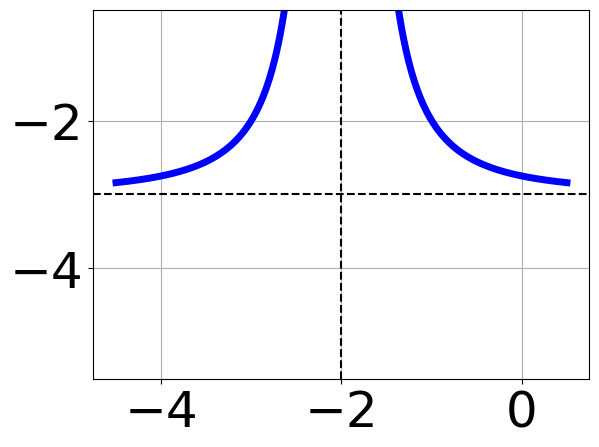
\includegraphics[width=0.5\textwidth]{../Figures/rationalGraphToEquationB.png}
\end{center}
\begin{enumerate}[label=\Alph*.]
\item \( f(x) = \frac{-1}{x + 2} - 3 \)
\item \( f(x) = \frac{-1}{(x + 2)^2} - 3 \)
\item \( f(x) = \frac{1}{x - 2} - 3 \)
\item \( f(x) = \frac{1}{(x - 2)^2} - 3 \)
\item \( \text{None of the above} \)

\end{enumerate} }
\litem{
Solve the rational equation below. Then, choose the interval(s) that the solution(s) belongs to.\[ \frac{-4x}{-6x + 5} + \frac{-6x^{2}}{-30x^{2} +x + 20} = \frac{-2}{5x + 4} \]\begin{enumerate}[label=\Alph*.]
\item \( \text{All solutions lead to invalid or complex values in the equation.} \)
\item \( x \in [-1.41,-1.22] \)
\item \( x_1 \in [0.19, 0.87] \text{ and } x_2 \in [-0.9,1.7] \)
\item \( x_1 \in [0.19, 0.87] \text{ and } x_2 \in [-4.7,-0.5] \)
\item \( x \in [-0.9,-0.56] \)

\end{enumerate} }
\litem{
Solve the rational equation below. Then, choose the interval(s) that the solution(s) belongs to.\[ \frac{40}{20x -35} + 1 = \frac{40}{20x -35} \]\begin{enumerate}[label=\Alph*.]
\item \( x \in [0.75,4.75] \)
\item \( x_1 \in [0.75, 2.75] \text{ and } x_2 \in [0.75,4.75] \)
\item \( \text{All solutions lead to invalid or complex values in the equation.} \)
\item \( x \in [-1.75,-0.75] \)
\item \( x_1 \in [-1.75, -0.75] \text{ and } x_2 \in [0.75,4.75] \)

\end{enumerate} }
\litem{
Choose the graph of the equation below.\[ f(x) = \frac{1}{(x - 2)^2} + 3 \]\begin{enumerate}[label=\Alph*.]
\begin{multicols}{2}\item 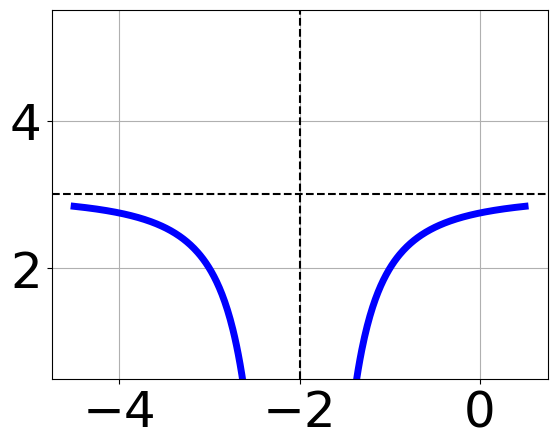
\includegraphics[width = 0.3\textwidth]{../Figures/rationalEquationToGraphAB.png}\item 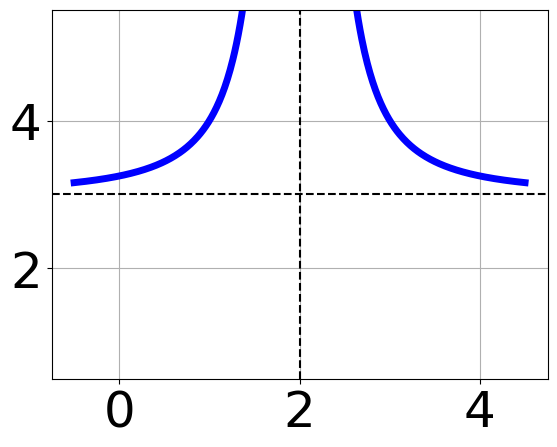
\includegraphics[width = 0.3\textwidth]{../Figures/rationalEquationToGraphBB.png}\item 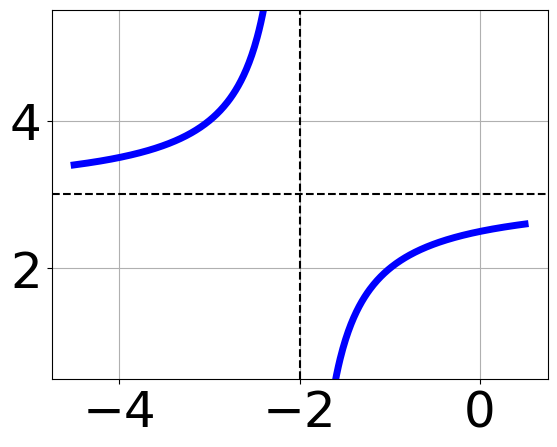
\includegraphics[width = 0.3\textwidth]{../Figures/rationalEquationToGraphCB.png}\item 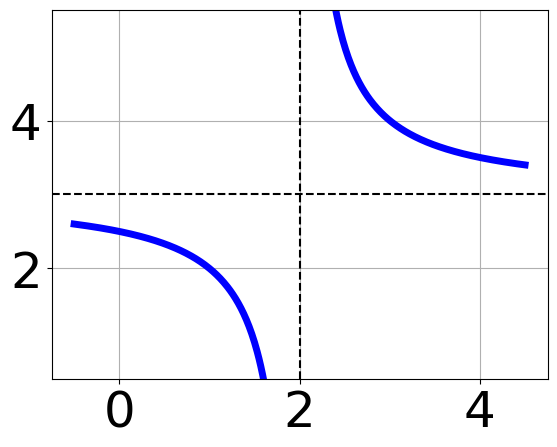
\includegraphics[width = 0.3\textwidth]{../Figures/rationalEquationToGraphDB.png}\end{multicols}\item None of the above.
\end{enumerate} }
\litem{
Solve the rational equation below. Then, choose the interval(s) that the solution(s) belongs to.\[ \frac{-7}{5x -9} + -6 = \frac{-2}{-30x + 54} \]\begin{enumerate}[label=\Alph*.]
\item \( \text{All solutions lead to invalid or complex values in the equation.} \)
\item \( x_1 \in [-3.04, 0.96] \text{ and } x_2 \in [1.47,1.59] \)
\item \( x \in [-3.04,0.96] \)
\item \( x \in [0.56,3.56] \)
\item \( x_1 \in [0.56, 2.56] \text{ and } x_2 \in [1.57,1.92] \)

\end{enumerate} }
\litem{
Determine the domain of the function below.\[ f(x) = \frac{3}{36x^{2} +48 x + 15} \]\begin{enumerate}[label=\Alph*.]
\item \( \text{All Real numbers except } x = a \text{ and } x = b, \text{ where } a \in [-30.12, -29.31] \text{ and } b \in [-18.17, -17.5] \)
\item \( \text{All Real numbers except } x = a, \text{ where } a \in [-30.12, -29.31] \)
\item \( \text{All Real numbers except } x = a, \text{ where } a \in [-0.86, -0.54] \)
\item \( \text{All Real numbers except } x = a \text{ and } x = b, \text{ where } a \in [-0.86, -0.54] \text{ and } b \in [-0.73, 0.03] \)
\item \( \text{All Real numbers.} \)

\end{enumerate} }
\litem{
Choose the graph of the equation below.\[ f(x) = \frac{1}{(x - 1)^2} + 2 \]\begin{enumerate}[label=\Alph*.]
\begin{multicols}{2}\item 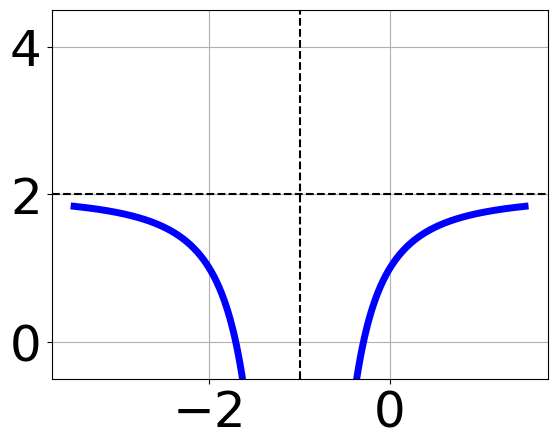
\includegraphics[width = 0.3\textwidth]{../Figures/rationalEquationToGraphCopyAB.png}\item 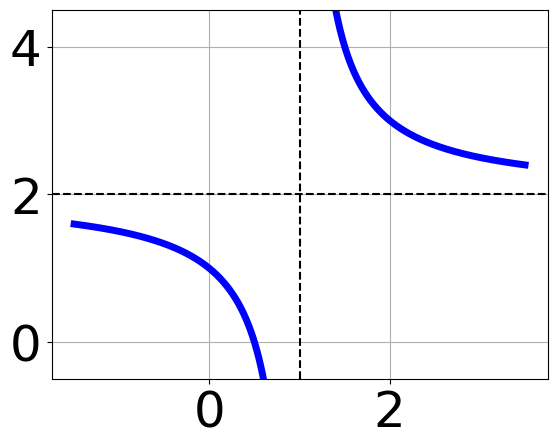
\includegraphics[width = 0.3\textwidth]{../Figures/rationalEquationToGraphCopyBB.png}\item 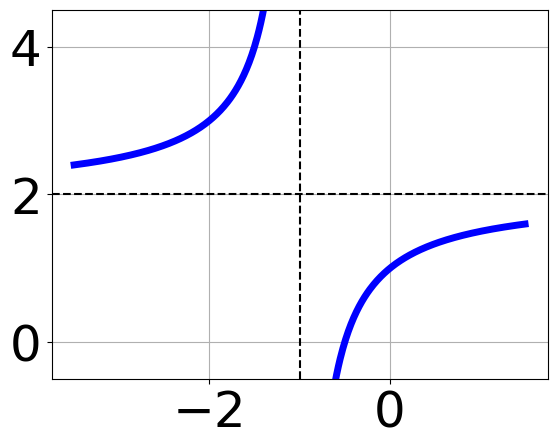
\includegraphics[width = 0.3\textwidth]{../Figures/rationalEquationToGraphCopyCB.png}\item 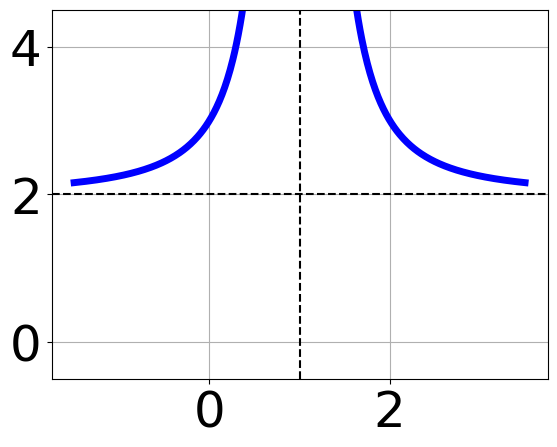
\includegraphics[width = 0.3\textwidth]{../Figures/rationalEquationToGraphCopyDB.png}\end{multicols}\item None of the above.
\end{enumerate} }
\litem{
Choose the equation of the function graphed below.
\begin{center}
    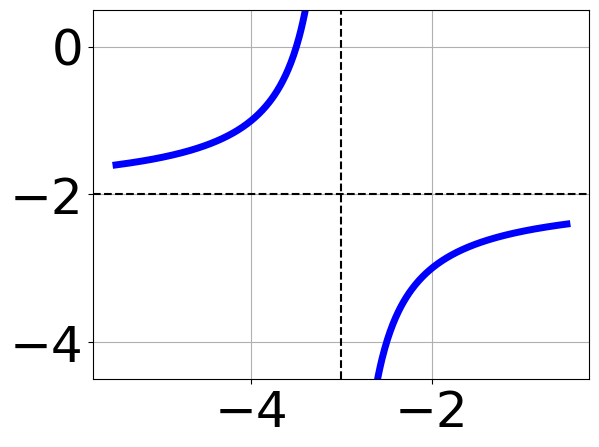
\includegraphics[width=0.5\textwidth]{../Figures/rationalGraphToEquationCopyB.png}
\end{center}
\begin{enumerate}[label=\Alph*.]
\item \( f(x) = \frac{1}{(x - 3)^2} - 4 \)
\item \( f(x) = \frac{-1}{x + 3} - 4 \)
\item \( f(x) = \frac{-1}{(x + 3)^2} - 4 \)
\item \( f(x) = \frac{1}{x - 3} - 4 \)
\item \( \text{None of the above} \)

\end{enumerate} }
\litem{
Solve the rational equation below. Then, choose the interval(s) that the solution(s) belongs to.\[ \frac{-2x}{2x -7} + \frac{-3x^{2}}{-10x^{2} +25 x + 35} = \frac{-3}{-5x -5} \]\begin{enumerate}[label=\Alph*.]
\item \( x \in [-1.69,0.55] \)
\item \( x_1 \in [0.01, 1.5] \text{ and } x_2 \in [0.5,4.5] \)
\item \( \text{All solutions lead to invalid or complex values in the equation.} \)
\item \( x \in [-3.37,-1.37] \)
\item \( x_1 \in [0.01, 1.5] \text{ and } x_2 \in [-6.22,2.78] \)

\end{enumerate} }
\end{enumerate}

\end{document}